
\section{Calibration Quality}\label{appendix:calib}
We perform post-hoc calibration using the default \texttt{CalibratedClassifierCV} in \texttt{sklearn.calibration}.
\cref{fig:appendix:calib} shows the reliability diagrams  (similar to those in \citet{kull2019beyond}) after calibration for \methodnamePrompt.
The resulting probabilities are overall quite calibrated.


\def \FigCalibration{
\begin{figure*}[ht]
\centering
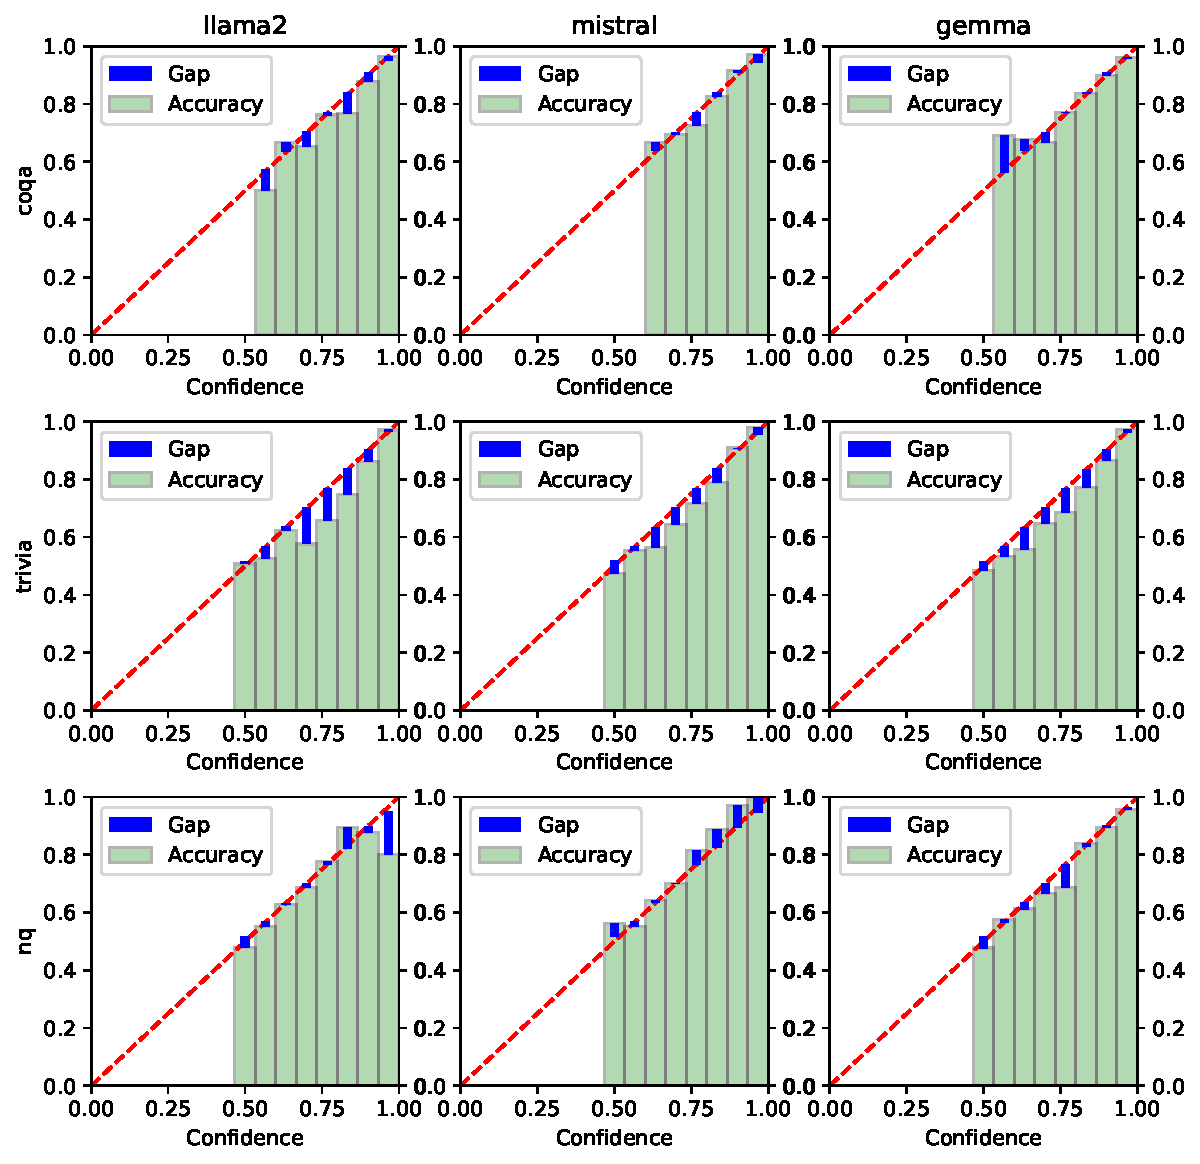
\includegraphics[width=0.8\textwidth]{Figures/reliability_diagrams.pdf}
\caption{
Reliability diagrams of \methodnamePrompt.
Bins with fewer than 10 samples are ignored due to noise.
}
\label{fig:appendix:calib}
\end{figure*}
}
\FigCalibration
